\chapter{Analyse fonctionnelle}

Le présent chapitre contient une présentation de l'ensemble des fonctions attendues du système, les différents acteurs qui interagiront avec celui-ci, ainsi que la répartition des responsabilités de chaque acteur par rapport aux différentes fonctionnalités. Une partie est également consacrée pour analyser l'état de l'existant et son positionnement vis-à-vis le besoin analysé. \\

\noindent La collecte, l'organisation, et la prioritisation des fonctions s'est basée sur l'analyse d'un document d'expression de besoin fourni par la fonction Conformité du Crédit Populaire du Maroc (CPM), ainsi qu'un nombre de réunions effectuées avec les représentants de cette fonction. \\

\clearpage



\section{État de l'existant}
Initialement, le registre de traitement utilisé par la banque existait sous forme de 80 fiches de traitement réparties sur 26 fichiers Excel. L'ajout, la modification, la consultation, et la validation des fiches de traitements se faisaient manuellement en manipulant des fichiers Excel qui faisaient l'objet de plusieurs transferts par mail entre les différents acteurs impliqués dans les processus liées à la gestion du registre de traitement. Bien que cette approche permettait à la banque de maintenir une certaine visibilité sur l'ensemble de ses traitements des donnnées à caractère personnel, elle présentait certaines lacunes et difficultées dont les plus impactantes étaient: \\

\noindent \textbf{Structure non standardisée}:
\begin{itemize}
    \item \textbf{Variabilité de format}: Les fichiers Excel peuvent avoir des structures différentes, ce qui complique l'importation automatisée.
    \item \textbf{Absence de normalisation}: Les entités peuvent ne pas suivre un schéma cohérent d'un fichier à l'autre, rendant difficile la définition d'un modèle de données uniforme.
\end{itemize}
\vspace{.4cm}
\noindent \textbf{Problèmes de qualité de données}:
\begin{itemize}
    \item \textbf{Données manquantes ou incomplètes}: Certains champs importants peuvent être vides ou mal remplis.
    \item \textbf{Données incohérentes}: Il peut y avoir des incohérences dans les valeurs (par exemple, des formats de dates différents, des fautes de frappe).
    \item \textbf{Erreurs de saisie}: Les données saisies manuellement sont sujettes à des erreurs humaines, ce qui peut affecter la qualité des informations.
\end{itemize}
\vspace{.4cm}

\noindent \textbf{Limitations techniques}:
\begin{itemize}
    \item \textbf{Taille des fichiers}: Les fichiers Excel volumineux peuvent poser des problèmes de performance lors de leur lecture et traitement;
    \item \textbf{Dépendance à un logiciel}: L'accès aux fichiers Excel nécessite souvent l'utilisation d'un logiciel spécifique (Microsoft Excel ou un équivalent), ce qui peut limiter la portabilité.
\end{itemize}
\vspace{.4cm}

\noindent \textbf{Gestion des versions}:
\begin{itemize}
    \item \textbf{Multiples versions}: La gestion de plusieurs versions des fichiers peut entraîner des problèmes de synchronisation et de traçabilité des modifications.
    \item \textbf{Absence de contrôle de version}: Il peut être difficile de suivre les modifications apportées aux fichiers, surtout si plusieurs personnes y ont accès.
\end{itemize}
\vspace{.4cm}

\mycomment{
\noindent \textbf{Sécurité et confidentialité}:
\begin{itemize}
    \item \textbf{Accès non sécurisé}: Les fichiers Excel peuvent être partagés sans contrôle d'accès strict, posant des risques pour la confidentialité des données.
    \item \textbf{Données sensibles}: Les fichiers peuvent contenir des informations sensibles nécessitant des mesures de sécurité supplémentaires.
\end{itemize}
\vspace{.4cm}


\vspace{.4cm}
\noindent \textbf{Mise à jour et maintenance}:
\begin{itemize}
    \item\textbf{Complexité de la mise à jour} : Mettre à jour les données ou corriger les erreurs dans les fichiers Excel peut être laborieux et sujet à des erreurs supplémentaires.
    \item \textbf{Maintenance difficile} : La maintenance des fichiers Excel (comme l'ajout de nouvelles colonnes ou la modification de la structure) peut être complexe et nécessiter des ajustements fréquents de l'application.
\end{itemize}
\vspace{.4cm}

\noindent \textbf{Performance et scalabilité}:
\begin{itemize}
    \item \textbf{Temps de traitement}: Le traitement des données à partir de fichiers Excel peut être lent, surtout si les fichiers sont volumineux ou nombreux.
    \item \textbf{Problèmes de scalabilité}: Les fichiers Excel ne sont pas conçus pour gérer de grandes quantités de données de manière efficace et peuvent poser des problèmes lorsque le volume de données augmente.
\end{itemize}
\vspace{.4cm}
}

\clearpage

\section{Spécification des besoins}

\subsection{Besoins fonctionnels}
\vspace{.4cm}
\begin{itemize}
    \item Tenir à jour le référentiel et la structure de registre de traitement; \vspace{.2cm}
    \item Saisir les données par fiche et selon la structure proposée en ligne et en colonne; \vspace{.2cm}
    \item Gérer la traçabilité des saisies, des modifications, et des actualisations des fiches de traitement; \vspace{.2cm}
    \item Gérer les relations et les renvois entre les fiches traitement; \vspace{.2cm}
    \item Recherches multicritères, par Catégorie de traitement, Sous-catégorie de traitement, traitement et/ou recommandation CNDP (ou Autorité locale pour les filiales à linternational); \vspace{.2cm}
    \item Centraliser lensemble des traitements des données à caractère personnel au sein de létablissement; \vspace{.2cm}
    \item Disposer d'un registre des traitements exhaustif, clair et facilement accessible; \vspace{.2cm}
    \item Avoir une vue densemble sur les traitements effectués par les entités de la BCP, et ce afin de mener une démarche damélioration continue dinventaire et de classification des données à caractère personnel; \vspace{.2cm}
    \item Faire revoir, compléter et valider facilement ces traitements par les RPO et Relais en charge de la protection des données personnelles.
\end{itemize}


\subsection{Besoins non-fonctionnels}

\begin{itemize}
    \item \textbf{Ergonomie:}
    \begin{itemize}
        \item Cohérence de l'interface: Par rapport aux attentes de l'utilisateur (facilité, simplicité, clarté, arrangement des écrans);
        \item Documentation implicite: En introduisant des Messages d'erreur ou d’accompagnement et un système d'aide en ligne;
        \item Facilité d'utilisation: Applicabilité de l'expérience de l'utilisateur dans un contexte analogue, réactions «naturelles» et intuitives;
        \item  Minimisation de la possibilité d'erreurs de manipulation: Offrir des listes déroulantes, choix des dates au lieu de les saisir, …etc; 
        \item  Minimisation de la possibilité d'erreurs de manipulation: Offrir des listes déroulantes, choix des dates au lieu de les saisir, …etc.
    \end{itemize}
    \item \textbf{Sécurité:} En plus de la sécurité qu'offre le système d'exploitation, l'application doit permettre:
    \begin{itemize}
        \item La gestion des habilitations concernant l'accés et l'utilisation de l'application;
        \item La gestion du système d'habilitation doit être du ressort d'un administrateur de l'outil.
    \end{itemize}
\end{itemize}

\clearpage

\section{Acteurs du système}
La gestion du registre de traitement nécessite la collaboration étroite de plusieurs acteurs dont l'intéraction efficace est primordiale pour l'atteinte des objectifs qui constituent la raison d'être du registre de traitement: \\

\begin{itemize}
    \item \textbf{Expert métier:} Il s'agit de l'acteur le plus familiarisé avec les traitements de données. Il peut être impliqué pour fournir des connaissances spécifiques sur la manière dont les données sont collectées, traitées et utilisées dans une activité ou un processus particulier; \\
    \item \textbf{Délégué à la protection des données (DPO):} Également appelé Data Protection Officer, il est chargé d'assurer la conformité aux réglementations en matière de protection des données au sein d'une organisation. Sa mission principale est d'informer et de conseiller l'organisme, de contrôler le respect du présent réglement et de coopérer avec les autorités de contrôle;\\
    \item \textbf{Relais de Protection des données Opérationnelle (RPO):} Sa responsabilité est d'effectuer un premier niveau de validation pour les fiches de traitement des donnnées;\\
    \item \textbf{Global Data Protection Officer (GDPO):} Il opère à l'échelle mondiale dans une organisation internationale. Il s'assure que les pratiques de protection des données sont cohérentes dans toutes les filiales de l'entreprise, en tenant compte des réglementations spécifiques à chaque juridiction. \\ \\
\end{itemize}


\noindent La collaboration entre l'expert métier, le Délégué à la Protection des données (DPO), le Relais de Protection des données Opérationnelle (RPO), et le Global Data Protection Officer (GDPO) est essentielle. Cette synergie vise à garantir la conformité et la cohérence des pratiques de protection des données, permettant ainsi d'atteindre les objectifs du registre de traitement.







\clearpage


\section{Cas d'utilisations}

\subsection{Diagramme de cas d'utilisation global simplifé}
\begin{figure}[H]
    \centering
    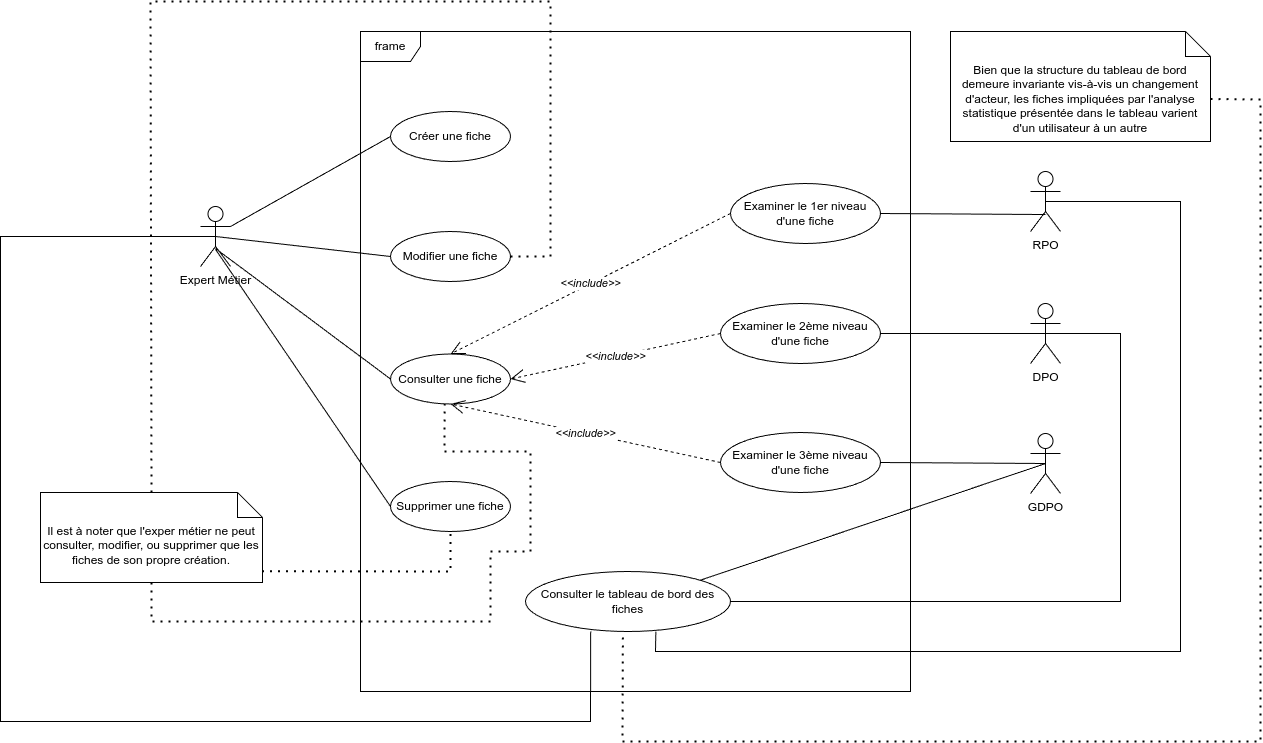
\includegraphics[width=\textwidth]{images/use-case.png}
    \caption{Diagramme de cas d'utilisation global simplifié}
\end{figure}


\subsection{Diagramme de cas d'utilisation de l'Expert métier}

\begin{figure}[H]
    \centering
    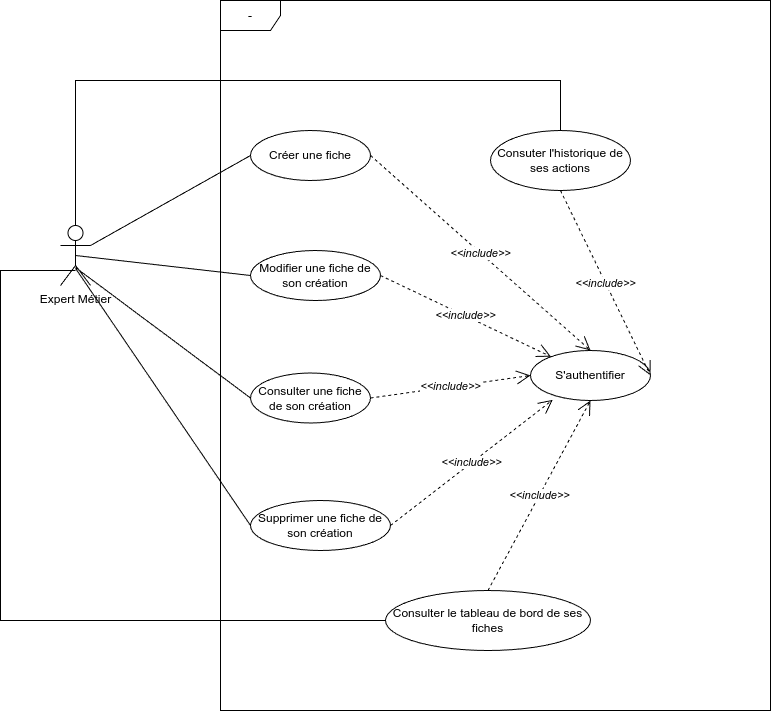
\includegraphics[width=\textwidth]{images/cas-utilisation-expert-metier.png}
    \caption{Diagramme de cas d'utilisation de l'expert métier}
\end{figure}

\clearpage


\subsection{Diagrammde de cas d'utilisation du RPO}

\begin{figure}[H]
    \centering
    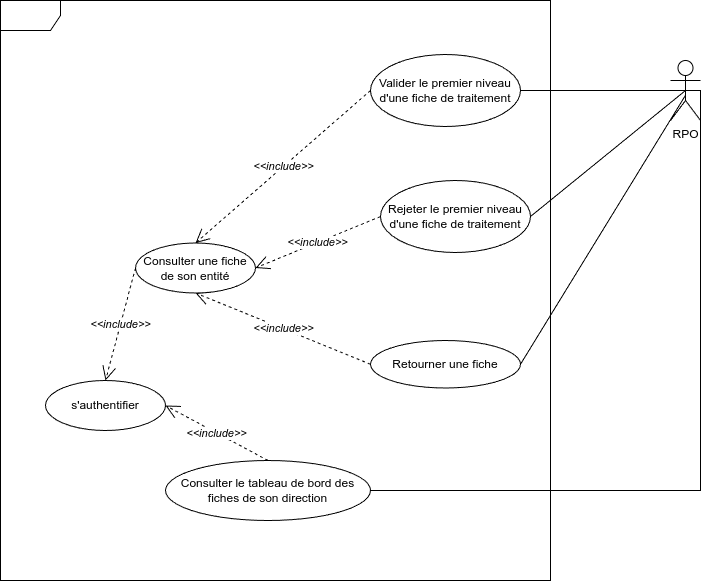
\includegraphics[width=\textwidth]{images/cas-utilisation-rpo.png}
    \caption{Diagrammde de cas d'utilisation du RPO}
\end{figure}

\clearpage

\subsection{Diagramme de cas d'utilisation du DPO}

\begin{figure}[H]
    \centering
    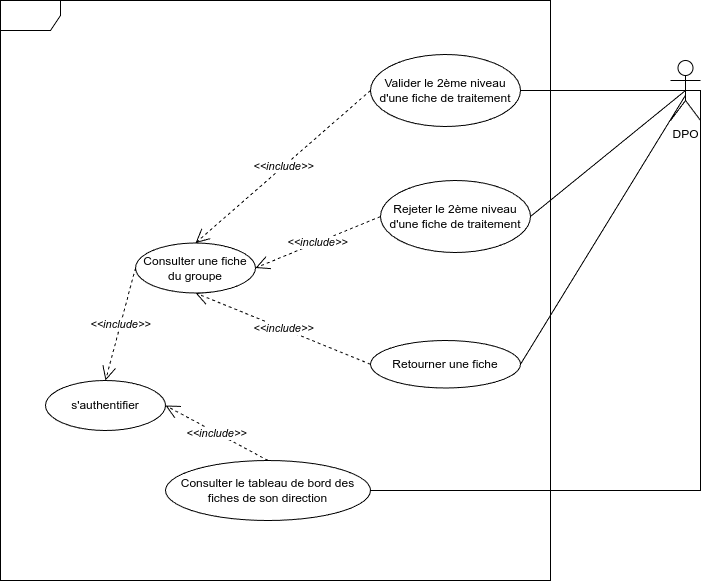
\includegraphics[width=\textwidth]{images/cas-utilisation-dpo.png}
    \caption{Diagramme de cas d'utilisation du DPO}
\end{figure}

\clearpage


\subsection{Diagramme de cas d'utilisation du GDPO}

\begin{figure}[H]
    \centering
    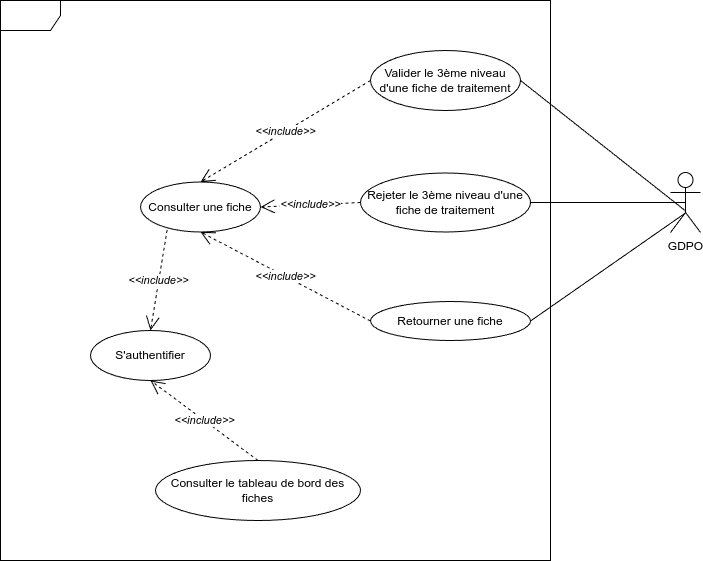
\includegraphics[width=\textwidth]{images/cas-utilisation-gdpo.png}
    \caption{Diagramme de cas d'utilisation du GDPO}
\end{figure}

\clearpage

\subsection{Diagramme de cas d'utilisation de l'agent d'habilitation}

\begin{figure}[H]
    \centering
    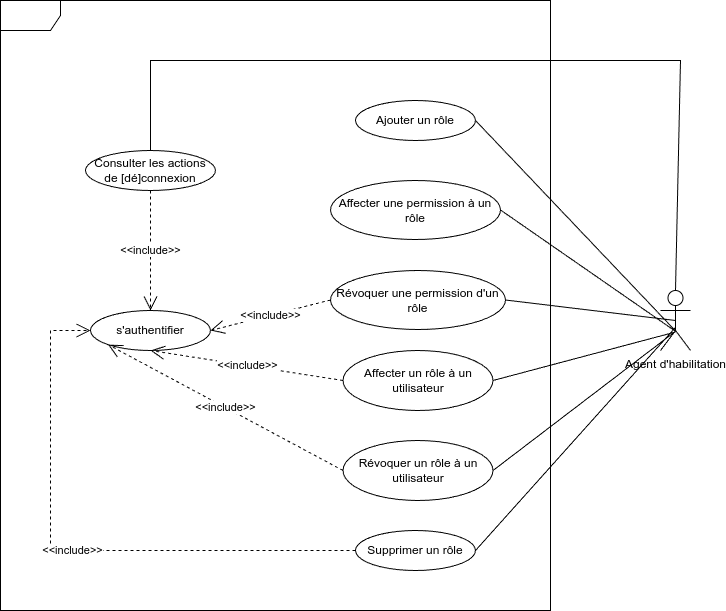
\includegraphics[width=\textwidth]{images/cas-utilisation-agent-habiliation.png}
    \caption{Diagramme de cas d'utilisation de l'agent d'habilitation}
\end{figure}



\clearpage